% Unused Apps

\documentclass[]{article}
\usepackage[utf8]{inputenc}
\usepackage{graphicx}
\usepackage[dvipsnames]{xcolor}
\usepackage[colorlinks=true,linkcolor=Blue,hypertexnames=false]{hyperref}
\usepackage{braket}
\usepackage{bbold}


\usepackage[numbers]{natbib}
\usepackage{amssymb}
\usepackage{amsmath}
\usepackage{placeins}
\usepackage{subcaption}
\usepackage[qm]{qcircuit}
\usepackage[left=23mm,right=23mm,top=35mm,columnsep=15pt]{geometry}

\usepackage{pgfplotstable}
\usepackage{array}

\newcommand{\caro}[1]{\textcolor{red}{[#1]}}
\newcommand{\jovan}[1]{\textcolor{blue}{[#1]}}
\newcommand{\todo}[1]{\textcolor{orange}{[#1]}}
\newcommand{\steve}[1]{\textcolor{purple}{[#1]}}
\newcommand{\lang}[1]{\textcolor{brown}{#1}}



\title{A proposal to demonstrate non-abelian anyons on a NISQ device}
\author{Jovan Jovanovi\'c, Carolin Wille, Daan Timmers and Steven H. Simon}
\date{February 2023}

\begin{document}

\section{Fusion and Braiding of Quantum Double Excitations}\label{app:fusion}\label{app:braid}

\textbf{Fusion.} In section \ref{sec:anyon}, we have mentioned that there is an algebra associated with irreducible representations of the quantum double algebra $D(G)$. In this appendix, we will derive the fusion coefficients that appear in this algebra
\begin{equation}
	a \otimes b = \bigoplus_c N_{ab}^x x,
\end{equation}
where labels $\{a,b,x\}$ are short versions of the full label of the irreducible representations, $x \equiv (C_x, \chi_x)$, where $C_x$ is some conjugacy class of the group $G$ and the $\chi_x$ is a irreducible representation of its centre.

The algebra above is completely analogous to the Clebsch-Gordan decomposition of the product of linear representations of a group into its irreducible representations. The number $N_{ab}^x$ numbers how many time does the representation $x$ appear in the product representations of $a$ and $b$.

To derive this quantity we start with the projector onto the representations $c$
\begin{equation}
	P^x = \frac{\chi_x(e)}{|Z(r_x)|}\sum_{c \in C_x}\sum_{z \in Z(r_x)}\chi_x^*(z)B_x^{(c)}A_x^{(q_c z \bar{q}_c)},
\end{equation}
where $q_c$ is a nonunique group element obeying $q_c c \bar{q}_c = r_x$, with $r_x$ as the $C_x$'s representative.

The matrices $A_x$ and $B_x$ in the equation above are the representation matrices in the $x$ irreducible representations, but the form of the projector is representation independent. We just need to figure out the their form in the $a\otimes b$ representation.

For this specific reason, the quantum double algebra is by definition equiped with a co-product operator
\begin{equation}\begin{split}
	\Delta(A_x^{(g)}) = A_a{(g)} \otimes A_b{(g)}\\
	\Delta(B_x^{(h)}) = \sum_{g \in G} B_a{(g)}\otimes B_b{(\bar{g}h)}.
\end{split}\end{equation}

After applying the co-product to the $x$-projector we arrive at the form of the projector in the $a\otimes b$ space
\begin{equation}
	P_{a \otimes b}^x = P_{ab}^x = \frac{\chi_x(e)}{|Z(r_x)|}\sum_{c \in C_x}\sum_{z \in Z(r_x)}\sum_{g\in G}\chi_x^*(z)B_a{(g)}A_b{(q_c z \bar{q}_c)}\otimes B_a{(\bar{g}c)}A_b{(q_c z \bar{q}_c)}.
\end{equation}
 The rank of this projector will be an integer multiple of the dimension of the $x$ representation and that integer is the fusion algebra coefficient $N_{ab}^x$.
 
 The more general way of calculating these fusion coefficients that is more familiar and is applicable for all anyon theories is the Verlinde formula
 \begin{equation}
 	N_{ab}^x = \sum_{l}\frac{S_{al}S_{bl}S^*_{cl}}{S_{0l}},
 \end{equation}
 where the sum is taken over all the anyon labels in the theory, the irreducible representations in our case. The matrix $S$ is the linking matrix and is defined, in terms of the planar diagram algera, as in the diagram in Figure \ref{fig:S_mat_def} (Left).
 \begin{figure}
 	\centering
 	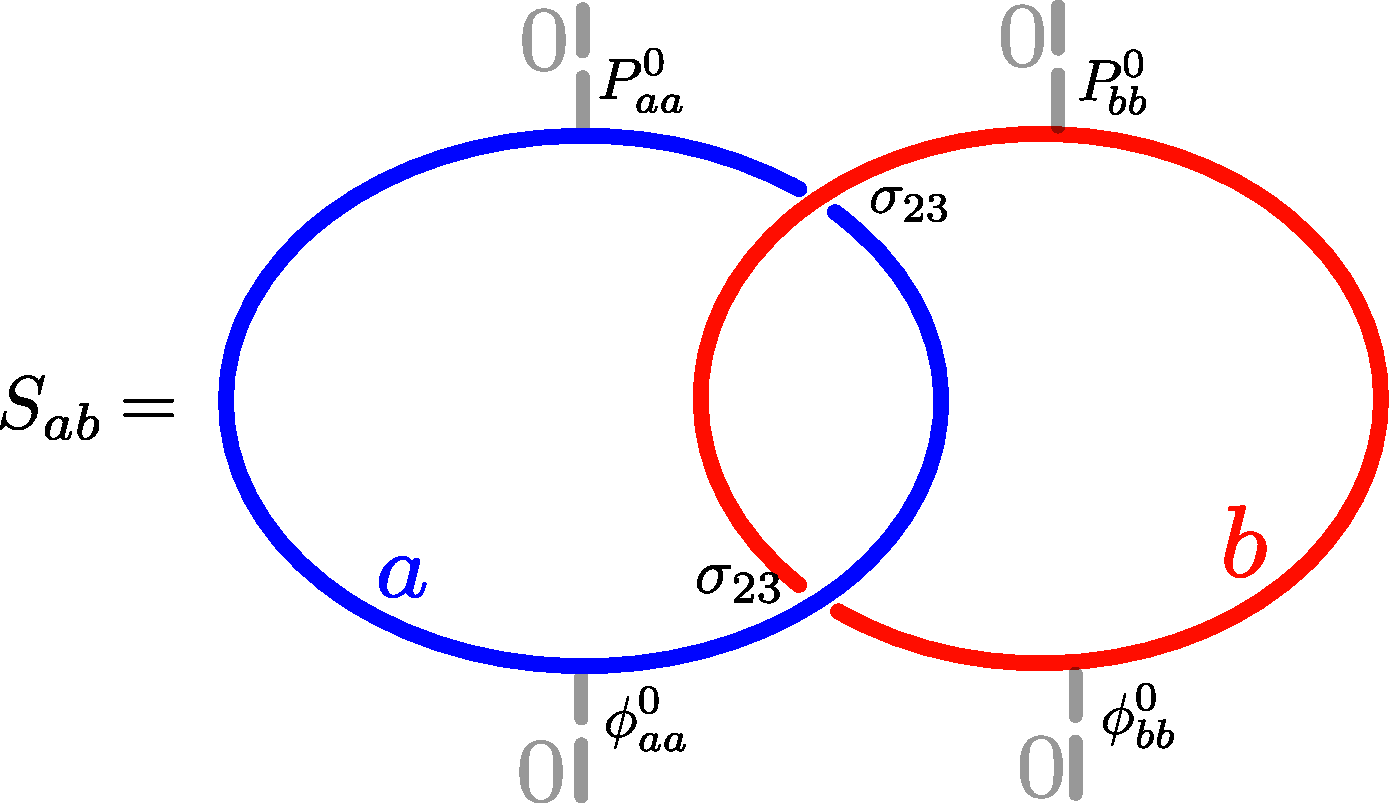
\includegraphics[width= 0.45\linewidth]{Figures/S_mat_def.pdf}\hspace{10pt}
 	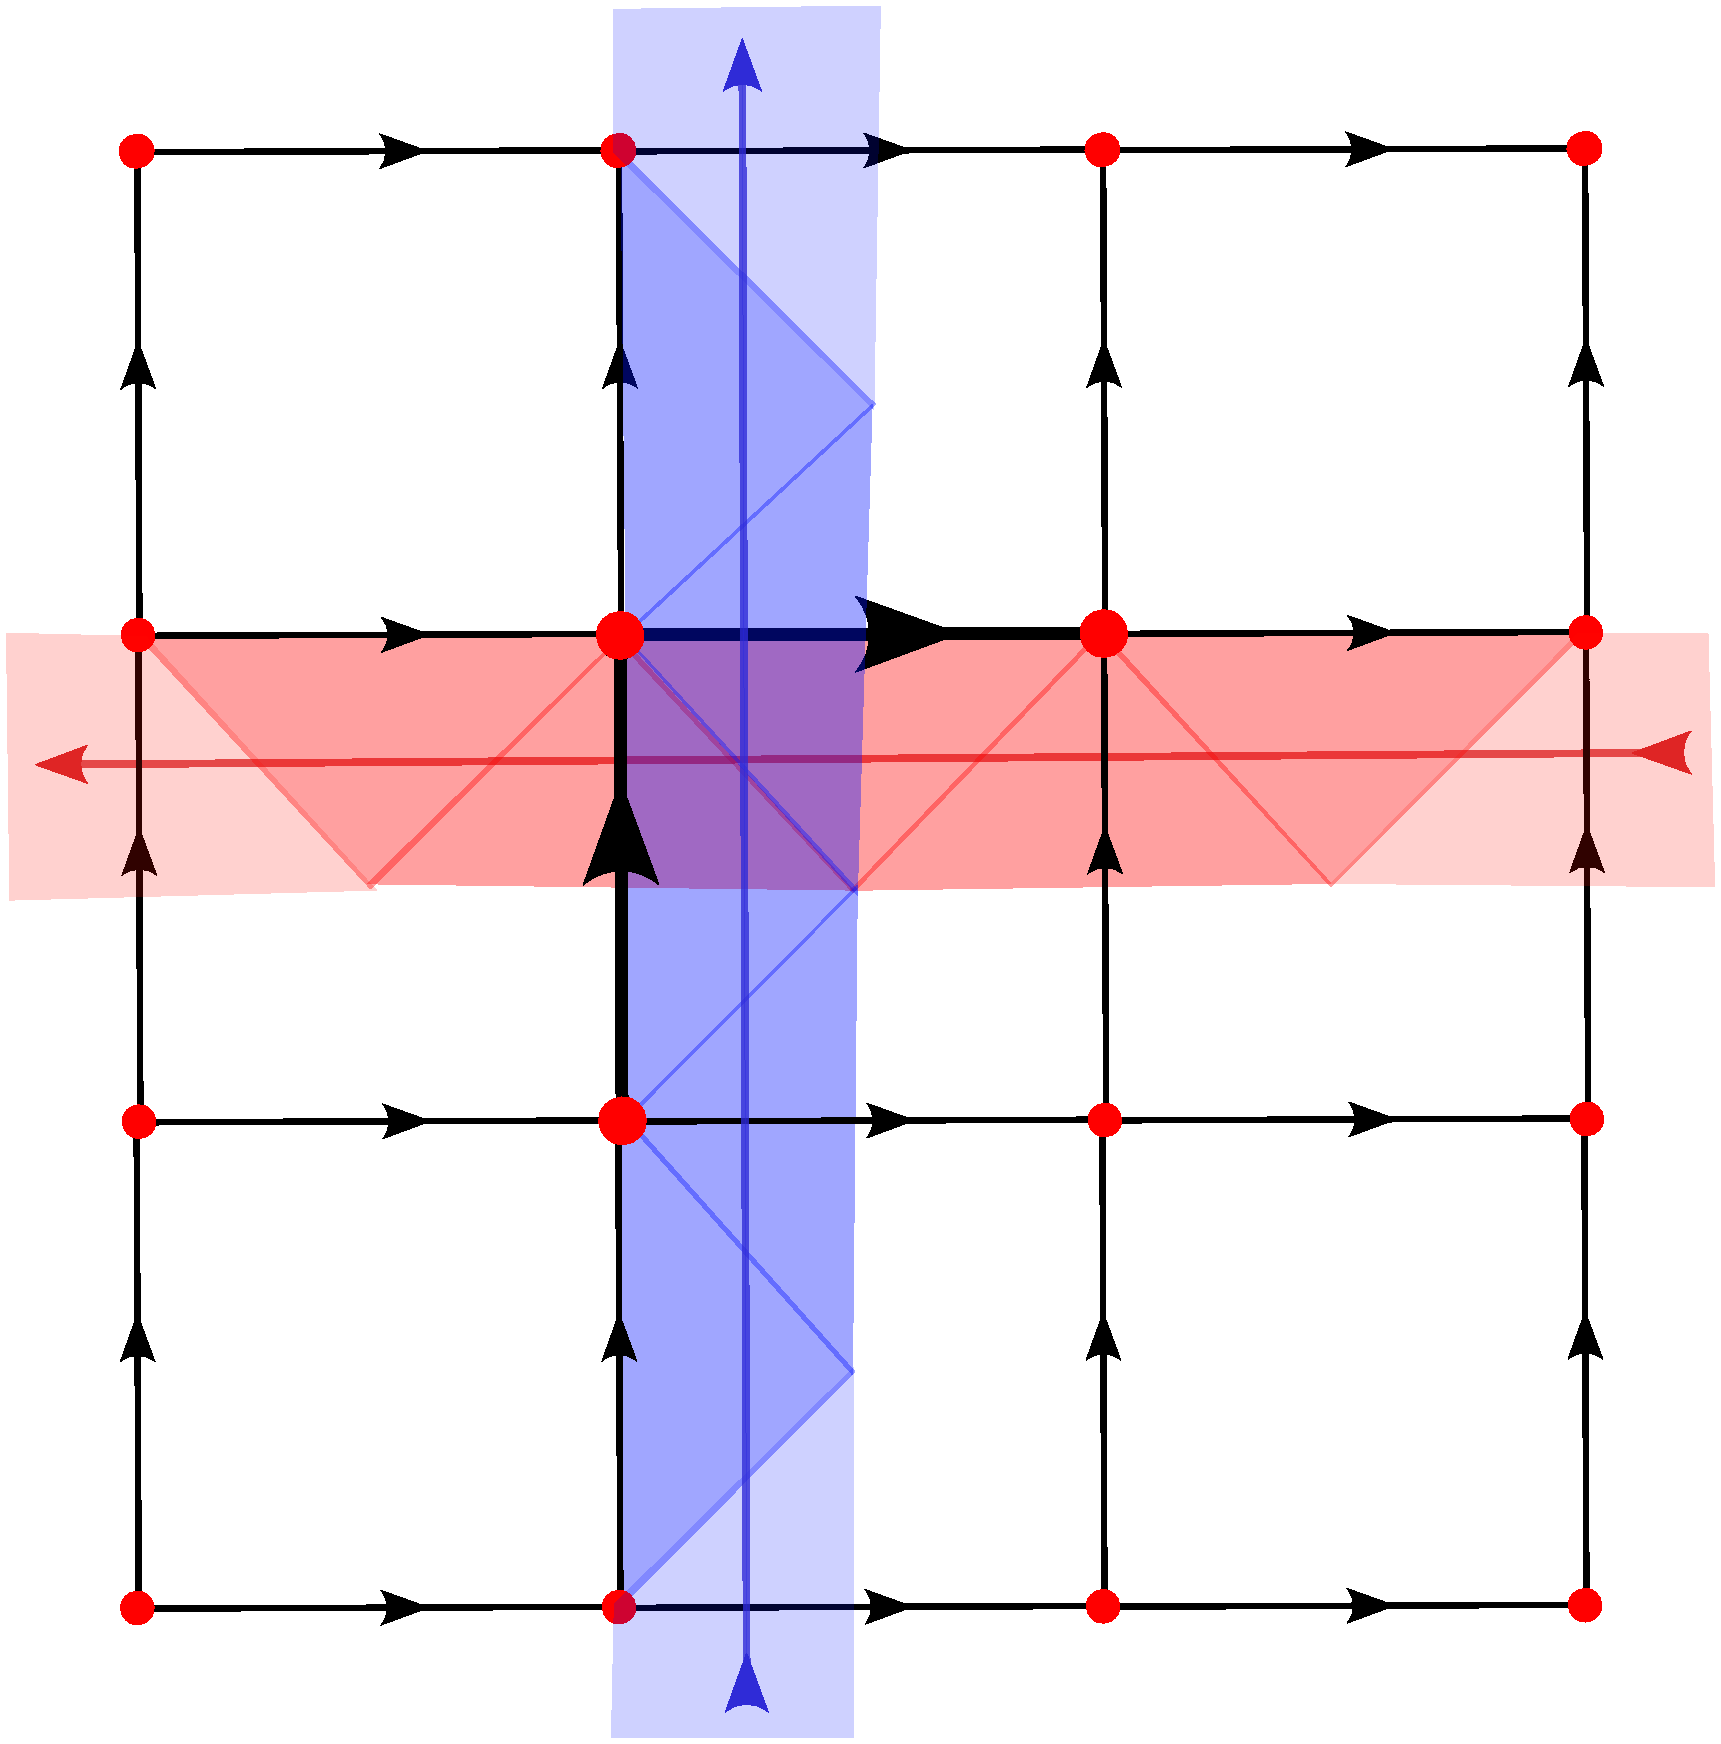
\includegraphics[width= 0.30\linewidth]{Figures/ribbon_crossing.pdf}
 	\caption{(Left) The diagram definition of the linking matrix elements between anyons $a$ and $b$ and its evaluation in the case of the quantum double model. $\sigma_{ii+1}$ represent the action of the braid group generator, the exchange of $i^{\text{th}}$ and $(i+1)^{\text{st}}$ anyon, on the representation space $a \otimes a \otimes b \otimes b$. $P_{xx}^0$ are projectors from the representation space $x \otimes x$ onto the trivial sector and $\phi_{xx}^0$ are functions whose inverses are these projectors. (Right) An example of ribbon crossing that arrises while braiding or annihilating the anyons. The two edges shared between the ribbons are marked in bold. Note that for each edge they share the ribbons have the opposite type of elementary triangle touching it; also that for each ribbon the triangles that touch the two shared edges are of opposite type.}
 	\label{fig:S_mat_def}
 \end{figure}
 
A well known result links the linking matrix of the quantum double model and the representation theory of the gauge group $G$
\begin{equation}
	S_{ab} = \frac{1}{|G|}\sum_{c_a \in C_a, c_b \in C_b, c_a c_b = c_b c_b} \chi_a(q_{c_a}^{-1}c_b q_{c_a})\chi_b(q_{c_b}^{-1}c_a q_{c_b}).\label{eqn:verlinde}
\end{equation}
 
 \textbf{Braiding. }In Figure \ref{fig:S_mat_def} (Left) we also shown how to derive Eq.~\eqref{eqn:verlinde} starting from the quantum double algebra representations, the only additional information we need is also provided by the definition of the quantum double algebra.
The action of the exchange of anyons on the product space is  given by
\begin{equation}
	\begin{split}
		\boldmath{\sigma}_{i i+1}: a_1 \otimes \ldots \otimes a_i \otimes a_{i+1} \otimes \ldots \otimes a_n \rightarrow a_1 \otimes \ldots \otimes a_{i+1} \otimes a_{i} \otimes \ldots \otimes a_n,\\
		\boldmath{\sigma}_{i i+1} = \mathbb{1} \otimes \ldots (\text{Flip } \circ \sum_{h \in G} A_i{(h)}\otimes B_{i+1}{(h)}) \otimes \ldots \otimes \mathbb{1},
	\end{split}
\end{equation}
with Flip operator denoting the trivial exchange of vector spaced in the tensor product. One can easily check that the exchange operators defined on this space obey the group multiplication rule of the braid group generators
$$\sigma_{i,i+1}\sigma_{i+1,i+2}\sigma_{i, i+1} =\sigma_{i+1,i+2}\sigma_{i,i+1}\sigma_{i+1, i+2}, $$
hence, it is a representation of the braid group on the product space.

Note that when we do the exchange of actual anyons in our system with the ribbon operators defined in Section \ref{sec:ribbon_ops} this action of the braid group generator is implemented.
The key is that once we perform the braiding (create, exchange and annihilate the anyons) the ribbons of the two exchanged anyons will cross, see Figure \ref{fig:S_mat_def} (Right).
The crossing ribbons share two edges and on these two edges the types of their elementary triangles are opposite, furthermore, the looking at each ribbon individually the the two elementary triangles touching the two edges are also opposite. This remains true even for irregular graphs.

The consequence of this geometrical fact on our protocol is that once the first ribbon traverses the shared edges it will multiply its edge label by it's own flux. And when the second ribbon crosses the edge that the first have had traversed the group action on the auxiliary qudit is shifter by this flux compared to the case where it was traversing the vacuum. This is exactly the required braiding action on the internal space of the anyons
\begin{equation}
	\sigma_{i,i+1}\ket{c, i}_i\ket{c', i'}_{i+1} = \sum_{h \in G}B_{i+1}{(h)}\ket{c',i'}_{i+1} A_i{(h)}\ket{c,i}_i = \ket{c',i'}_{i+1} A_i{(c')}\ket{c,i}_{i}. 
\end{equation}


%\subsection{Fusion rules of $D(D_4)$}
%The existence of multiple fusion outcomes is the defining property for non-Abelian anyons and probed in two of our protocols. The fusion of two identical non-Abelian pure fluxes is given by
%
%\begin{equation}
%\begin{aligned}
%	 \Psi_i \times  \Psi_i =  O + \tilde O +  \Sigma_i + \tilde \Sigma_{i}	 \;.	
%	 \end{aligned}
%	\end{equation}
%For different non-Abelian pure fluxes, we have
%\begin{equation}
%	\Psi_r \times \Psi_{m} = \Psi_{mr}+\tilde \Psi_{mr} \;, \quad \Psi_r \times \Psi_{mr} = \Psi_m + \tilde \Psi_m \;, \quad \Psi_m \times \Psi_{mr} = \Psi_r + \Phi_r \;.
%\end{equation}	
%

\section{Post-selection probabilities}\label{app:postsel}
In this appendix, we will elaborate on the post-selection probabilities quoted in the main text.

Any quantum algorithm that includes post-selection invokes a justified concern about the post-selection success rates and scaling of the needed number of ruins to build up a valid statistical sample of successful runs.

In the main text we have mentioned that the post-selection on the Bell pair measurements on the ribbon application auxiliary qubits is $1/4$ if the ribbon is open and $1$ if it's closed, and we are applying them on the ground state.

If we apply our protocol on a product state $\ket{\{g\}}$, we get that the probability of the Bell pair measurement succeeding is $$ p = |\frac{1}{2}\text{Tr}A(g_1 g_2 \ldots g_n)|^2,$$ where the group elements $g_i$, for $i \in \{1,\ldots n\}$, are the group element labels of the edges crossed by the ribbon, in the order of crossing, as defined by the product state $\ket{\{g\}}$.

If we wish to apply this analysis for the ground state, we have to trace out the gauge field, expect for this non-trivial degree of freedom $g_t = g_1 g_2 \ldots g_n$.

In terms of the newly acquired density matrix, $\rho_{g_t g_t'}$, the post-selection success probability is $$p = \sum_{g_t g_t'} \rho_{g_t g_t'} \frac{1}{2}\text{Tr}A^*(g_t)\frac{1}{2}\text{Tr}A(g_t').$$

Now, if the ribbon is open, the reduced density matrix is uniform $$\rho_{g_t g_t'} = \frac{1}{8}\delta_{g_t, g_t'},$$ because there are no finite range correlations.

However, if the ribbon is closed, beacuse we are in the ground state, that is a Gauss' law state, we know $g_t = e$. Hence, the reduced density matrix is $$\rho_{g_t g_t'} = \delta_{g_t, g_t'} \delta_{e, g_t}.$$

\jovan{Something is not adding up :(}

\end{document}
